\documentclass[10pt]{beamer}

\usetheme{metropolis}

\usepackage{graphicx}
\usepackage{subfig}
\usepackage{siunitx}
\usepackage{amsmath}

\newtheorem{mydef}{Definition}

\title{Special Relativity: Quirked Up, but Goated W/ Sauce}
\author{Duncan Wilkie}
\date{8 June 2022}

\begin{document}

\begin{frame}
  \titlepage
\end{frame}

\begin{frame}
  \frametitle{Foundation}
  Einstein derived the mathematical formalism of SR from two axioms:
  \begin{itemize}
  \item The laws of physics are the same in any coordinate system with the origin moving at constant velocity (i.e. \textit{there is no absolute rest})
  \item  The speed of light in the vacuum is constant
  \end{itemize}
\end{frame}

\begin{frame}
  \frametitle{Motivation}
  Why these axioms? Two reasons, as he explains in the eminently readable paper \textit{Zur Elektrodynamik bewegter Körper}:
  \begin{itemize}

  \item The observable characteristics of first mechanics and then electrodynamics just so happened to depend only on the relative motion of bodies.
  \item Despite the motion of Earth, the velocity of light appears to be isotropic.
  \end{itemize}
\end{frame}

\begin{frame}
  \frametitle{Motivation: Electrodynamics}
  To illustrate Einstein's first point, one needs a crash-course in electromagnetism.
  The subject is about two vector fields: $\vec{E}$, the electric field produced by charged particles, and $\vec{B}$, the magnetic field produced by moving charges.
  These fields affect the dynamics of charges by Coulomb's law
  \[
    \vec{F}= q(\vec{E}+\vec{v}\times\vec{B})
  \]

  Before Faraday, the subject was only "electrostatics:" the study of situations involving unchanging fields.
  The known laws were
  \[
    \nabla\cdot\vec{E} = \frac{1}{\epsilon_{0}}\rho \hspace{0.5in}  \textrm{(Gauss's law)}
  \]
  \[
    \nabla\times\vec{E}=0 \hspace{0.5in} \textrm{(}\vec{E}\textrm{ has a scalar potential)}
  \]
  \[
    \nabla \cdot \vec{B} = 0   \hspace{0.5in} \textrm{(No magnetic monopoles)}
  \]
  \[
    \nabla \times \vec{B} = \mu_{0}\vec{J} \hspace{0.5in} \textrm{(Amp\`ere's law)}
  \]
\end{frame}

\begin{frame}
  \frametitle{Motivation: Electrodynamics}
  Faraday, through pure, brute-force experimentation, deduced that \textit{a changing magnetic field induces an electric field}; mathematically,
  \[
    \nabla\times\vec{E}=-\frac{\partial\vec{B}}{\partial t} \hspace{0.5in}\textrm{(Faraday's law)}
  \]
  In terms of the voltage associated with this electric field in a wire loop, this is written
  \[
    \mathcal{E}=-\frac{d\Phi}{d t}
  \]
\end{frame}

\begin{frame}
  \frametitle{Motivation: Electrodynamics}
  Maxwell noted a mathematical inconsistency in these four fundamental equations. Take the divergence of Amp\`ere's law:
  \[
    \nabla\cdot(\nabla\times \vec{B})=\mu_{0}(\nabla\cdot\vec{J})
  \]
  It's an easy proof that for arbitrary $C^{2}$ fields $\vec{B}$ that the left side is zero (exercise). However, in almost every case with a changing current, the right side will be nonzero.
  Noting that by Gauss's law and conservation of charge $\nabla\cdot \vec{J}=-\nabla\cdot\left( \epsilon_{0}\frac{\partial\vec{E}}{\partial t} \right)$, Maxwell canceled off this nonzero term by modifying Amp\`ere's law to be
  \[
    \nabla\times\vec{B}=\mu_{0}\vec{J}+\mu_{0}\epsilon_{0}\frac{\partial \vec{E}}{\partial t}
  \]
  Despite being difficult to observe in the laboratory, this law can be confirmed with high-frequency AC sources (cf. Hertz 1888).
\end{frame}

\begin{frame}
  \frametitle{Motivation: Electrodynamics}
  Maxwell's correction has a very nice interpretation: just as Faraday says \textit{a changing magnetic field induces an electric field}, so \textit{a changing electric field induces a magnetic field}.

\end{frame}

\begin{frame}
  \frametitle{Motivation: Electrodynamics}
  Notice, however, that unlike classical mechanics, it is not at all obvious that a ``principle of relativity'' applies for electromagnetism.
  \[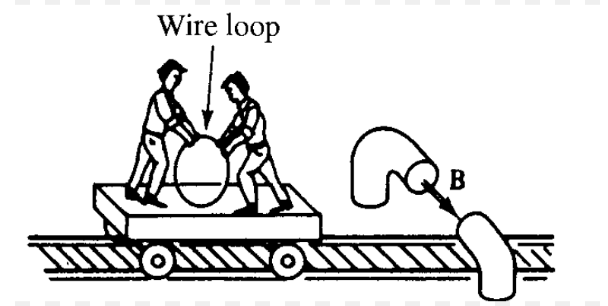
\includegraphics[scale=0.2]{train.png}\]
  In the situation pictured above, from the perspective of the ground, the force that creates a current is \textit{purely magnetic}; from the perspective of the train, it is \textit{purely electric}.
  It \textit{just so happens} that both perspectives yield the same voltage in the loop.

  Einstein conjectured that \textit{all physical theories} must give the same results when calculations are performed in inertial reference frames (coordinate systems moving at constant velocities).

\end{frame}

\begin{frame}
  \frametitle{Motivation: Electrodynamics}
  The primitive sources of electric and magnetic forces are point charges and line currents, respectively.
  These produce electric and magnetic fields (expressed in the natural cylindrical coordinates)
  \[
    \vec{E}=\frac{1}{4\pi\epsilon_{0}}\frac{q}{r^{2}}\hat{r}
  \]
  and
  \[
    \vec{B}=\frac{\mu_{0}I}{2\pi r}\hat{\theta}
  \]
  Each law depends on a phenomenological parameter: $\epsilon_{0}$, the permittivity of free space, and $\mu_{0}$, the permeability of free space.
  Qualitatively, these determine ``how easily'' electric and magnetic fields can travel through the vacuum: if $\epsilon_{0}$ is lower or $\mu_{0}$ higher, the fields fall off quicker in the limit $r\to\infty$.

  One can derive that for electromagnetic waves $\mu_{0}\epsilon_{0}=\frac{1}{c^{2}}$; it wouldn't make sense for either $\mu_{0}$ or $\epsilon_{0}$ to vary with speed (they're about propagation through the vacuum, after all!), so perhaps $c$ is fixed too.
\end{frame}


\begin{frame}
  \frametitle{Motivation: Michelson-Morley}
  In 1887, Michelson and Morley performed an experiment to try and find the speed of the Earth through ``the \ae ther,'' the conjectured medium through which electromagnetic waves propagate.
  Presumably, as with any other wave, the observed speed of light waves moving ``downstream'' from Earth in this medium would be the fastest.
  Through fancy interferometry, found an upper bound on that speed of \SI{\pm 6}{km/s}, despite the fact that with respect to the Sun we ought to be moving at \SI{30}{km/s}.
  \begin{center}
    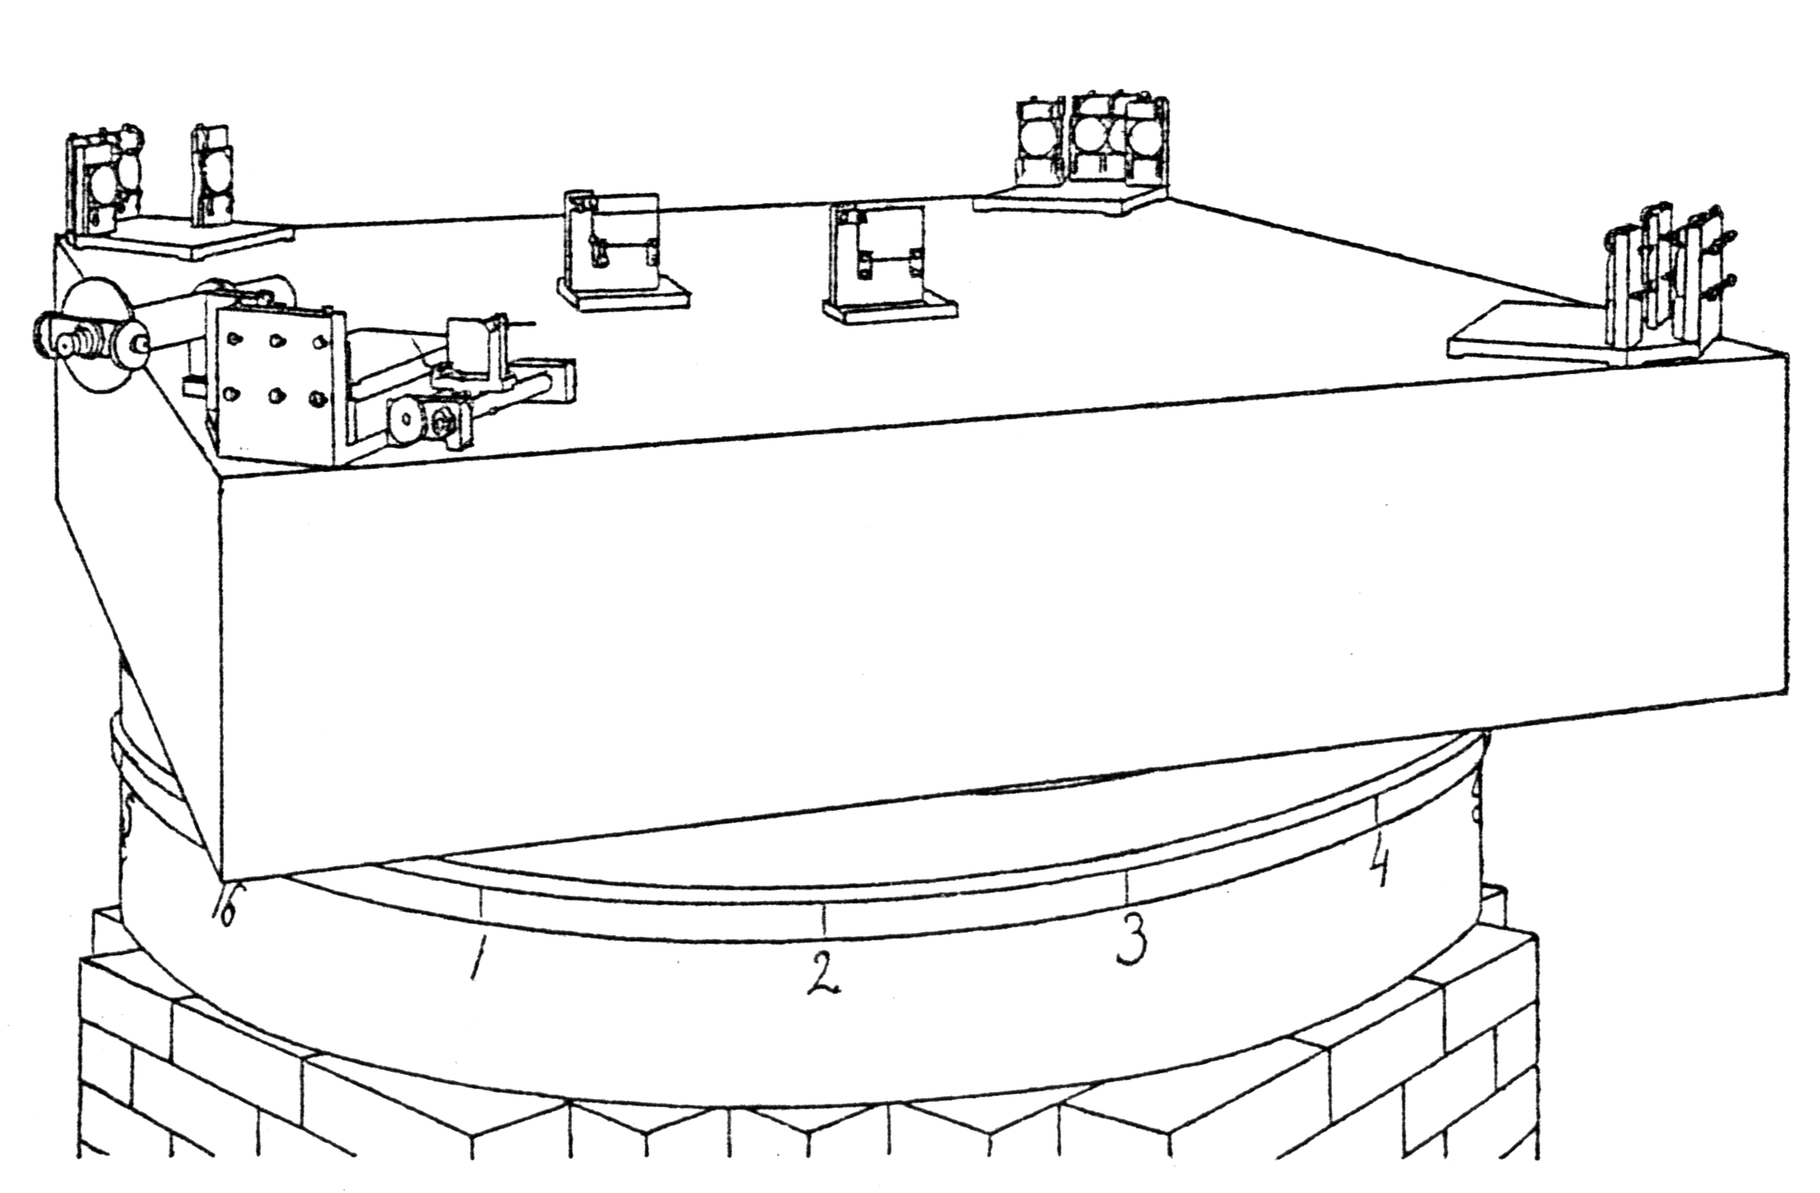
\includegraphics[scale=0.4]{mich-mor.png}
  \end{center}
  Thus Einstein conjectured that the speed of light in the vacuum is a universal constant.
  Modern measurements have gotten the estimate down to $\SI{e-7}{km/s}$, and introduced the universal frame candidate of the CMB, with respect to which we move around 10x faster.
\end{frame}

\begin{frame}
  \frametitle{Consequences: The Objective}
  Clearly, saying the speed of light is \textit{always} constant has drastic implications.
  If one is moving at the speed of light, the light one shines forward moves not at $2c$ but $c$.
  Speed is in units of \si{m/s}, and so we have two quantities to play with: we can change what ``meter'' means, i.e. lengths change, or what ``seconds'' means, i.e. time changes.
  It'll turn out to require both.
  In classical mechanics, an event located by coordinates $(t,x,y,z)$ has coordinates $(t',x',y',z')$ with respect to an origin moving with speed $v$ along the $x$-axis given by
  \[
    x'=x-vt
  \]
  \[
    y'=y
  \]
  \[
    z'=z
  \]
  \[
    t'=t
  \]

\end{frame}

\begin{frame}
  \frametitle{Consequences: The Objective}
  This is a linear mapping $\mathbb{R}^{4}\to\mathbb{R}^{4}$, and so may be expressed as a matrix with respect to the initial basis as
  \[
    \begin{pmatrix}
      1 & 0 & 0 & 0 \\
      -v & 1 & 0 & 0 \\
      0 & 0 & 1 & 0 \\
      0 & 0 & 0 & 1
    \end{pmatrix}
  \]
  (Check this by letting it act on the 4-vector $(t,x,y,z)$!)

  Our goal is to find an analogous mapping for which Einstein's axioms hold.
\end{frame}

\begin{frame}
  \frametitle{Consequences: Time Dilation}
  We start by trying to find the time transformation.
  Consider a light bulb on the roof of a moving train car, pictured below.
  \[
    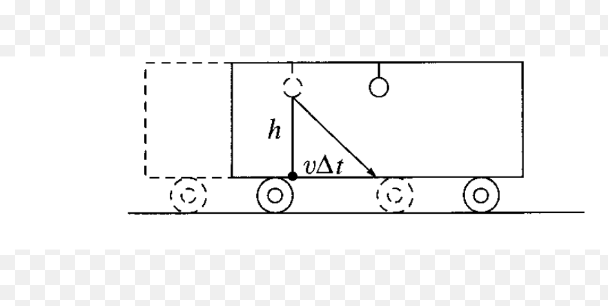
\includegraphics[scale=0.2]{time-dilation.png}
  \]
  For an observer in the car (coordinates distinguished via priming), the light moves straight down, and the time it takes to strike the ground is simply $\Delta t'=h/c$.
  For an observer on the ground, however, it travels a longer distance, and so takes the longer time $\Delta t=\sqrt{h^{2}+(v\Delta t)^{2}}/c$.
  Solving for $\Delta t$, one gets $\Delta t = \frac{h}{c}\frac{1}{\sqrt{1-v^{2}/c^{2}}}$.
  We then get the famous time dilation equation
  \[
    \Delta t' =\Delta t\sqrt{1-v^{2}/c^{2}}= \Delta t/\gamma \textrm{ (defining } \gamma)
  \]
\end{frame}

\begin{frame}
  \frametitle{Consequences: Length Contraction}
  Now we proceed similarly for length.
  Consider the same train car, but with the bulb on the back wall and a mirror on the front wall:
  \[
    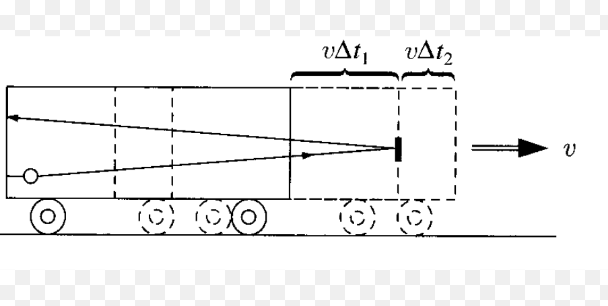
\includegraphics[scale=0.2]{length-contraction.png}
  \]
  What's the travel time of the light?
  On the train, this is again simply $\Delta t'=2\frac{\Delta x'}{c}$.
  On the ground it's more complicated.
  Letting $\Delta t_{1}=\frac{\Delta x+v\Delta t_{1}}{c}\Leftrightarrow \Delta t_{1}=\frac{\Delta x}{c-v}$ be the time to strike the mirror and $\Delta t_{2}=\frac{\Delta x-v\Delta t_{2}}{c}=\frac{\Delta x}{c+v}$
  be the time to strike the rear wall, the total time is $\Delta t=\Delta t_{1}\Delta t_{2}\frac{2\Delta x}{c}\frac{1}{1-v^{2}/c^{2}}$.
  We also have the time dilation formula; substituting these expressions of $\Delta t'$ and $\Delta t$ in terms of the displacement yields the length contraction formula
  \[
    \Delta x' = \frac{\Delta x}{\sqrt{1-v^{2}/c^{2}}} = \gamma\Delta x
  \]
\end{frame}

\begin{frame}
  \frametitle{Consequences: Lorentz Transformations}
  Note that $\gamma=\frac{1}{\sqrt{1-v^{2}/c^{2}}}<1$ for $v<c$.
  In summary, then, \textit{moving clocks run slow} and \textit{moving rulers get shorter}, both by a factor of $\gamma$.
  In principle, this is ``all'' of special relativity.
  In analogy to the Galilean transformations, we can write
  \[
    \Lambda = \Lambda_{\mu}^{\nu}
    \begin{array}{l}
      t' = \gamma\left( t-\frac{v}{c^{2}}x \right) \\
      x' = \gamma (x - vt) \\
      y' = y \\
      z' = z
    \end{array}
    \Leftrightarrow
    \begin{pmatrix}
      \gamma & -\gamma \frac{v}{c^{2}} & 0 & 0 \\
      -\gamma v & \gamma & 0 & 0 \\
      0 & 0 & 1 & 0 \\
      0 & 0 & 0 & 1
    \end{pmatrix}
  \]
  The $x'$ equation follows from length-contracting \textit{and} time-dilating the argument leading to the Galilean formula,
  and the $t'$ equation may be deduced by plugging the formula for transforming $x$ \textit{from} the primed frame \textit{to} the unprimed frame into that for $x'$.
  The matrix can be made Hermitian by taking the first component of the vectors it acts on be $ct$ instead of $t$.
\end{frame}

\begin{frame}
  \frametitle{4-Vectors and the Minkowski Metric}
  The Lorentz transformation acts on vectors with \textit{four} components.
  We distinguish between these \textit{spacetime} vectors (by convention with time as the first component) and ordinary space vectors by calling them 4-vectors, and using Greek indices when they're written in expressions.
  The analog of the dot product on 4-vectors is the same as $\mathbb{R}^{4}$, but with a negative first component:
  \[
    {a^{\mu}}\cdot{b^{\mu}}=-a^{0}b^{0}+a^{1}b^{1}+a^{2}b^{2}+a^{3}b^{3}
  \]
  Note the use of superscript indices; this is a critical point, as $a^{\mu}\neq a_{\mu}$, differing by the negation of the time component.
  As we'll see later, this is a metric tensor (the Minkowski metric) on the spacetime manifold.
\end{frame}

\begin{frame}
  \frametitle{Light Cones}
  Just as how $a\cdot a = |a|^{2}$ on $\mathbb{R}^{4}$, we can define the ``distance'' between two intervals in spacetime by the magnitude of their vector difference.
  An important distinction is that this ``distance'' can be negative; we can classify separations by the sign of this value.
  If it's positive, the separation is spacelike, if it's negative, timelike; zero, lightlike.
  These terms are motivated by inspecting so-called \textbf{light cones}: the points in the interior of the cone are spacelike, those on its boundary are lightlike, and the exterior is timelike.
  \begin{center}
    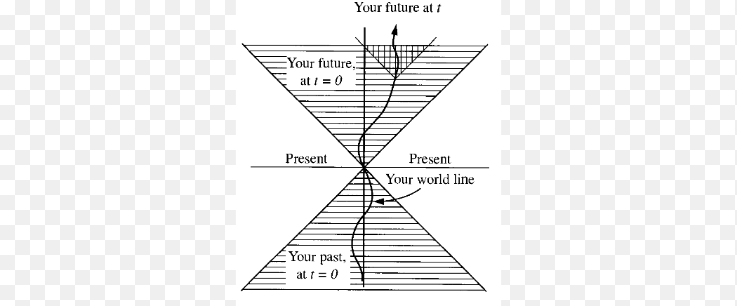
\includegraphics[scale=0.35]{lightcone.png}
  \end{center}
\end{frame}

\begin{frame}
  \frametitle{Fun Problems}
  \begin{figure}[!tbp]
    \centering
    \subfloat{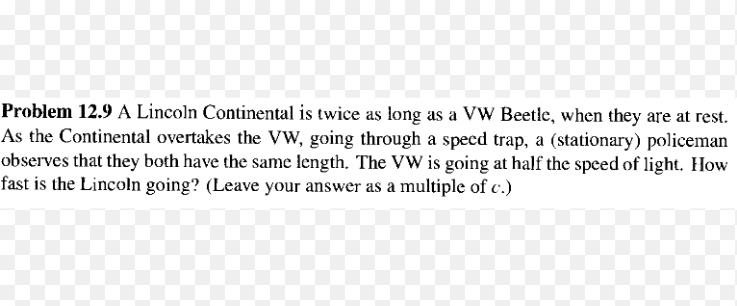
\includegraphics[scale=0.2]{ex1.png}}
    \hfill
    \subfloat{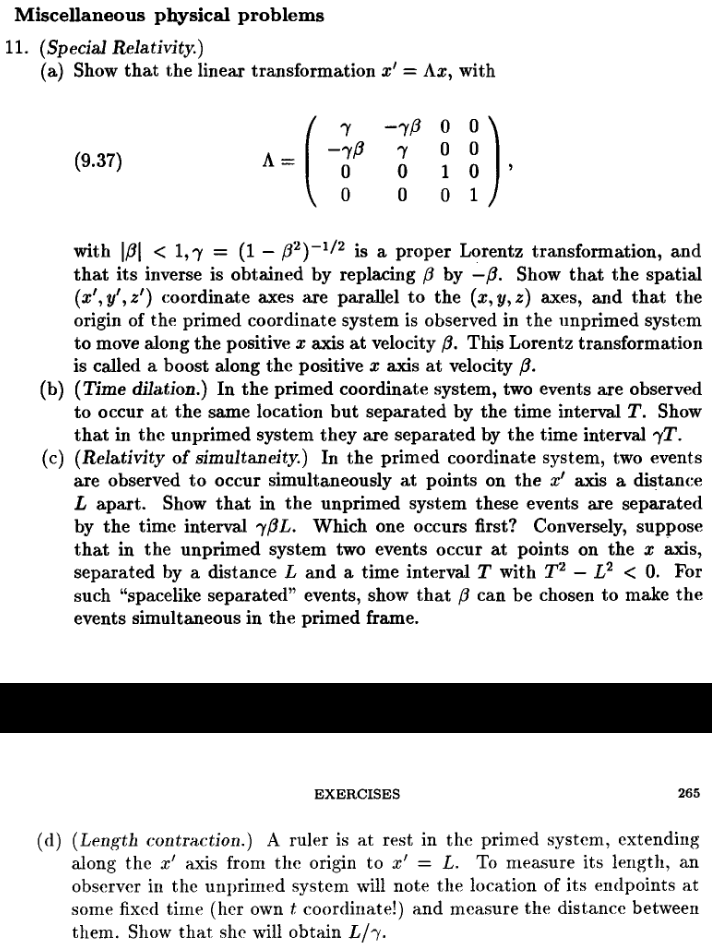
\includegraphics[scale=0.2]{ex2.png}}
  \end{figure}
\end{frame}

\begin{frame}
  \frametitle{Fun Paradoxes and Further Thinking}
  \begin{itemize}
  \item Relativity of simultaneity
  \item Twin paradox
  \item Ladder paradox
  \item Shadows move faster than light
  \end{itemize}
\end{frame}

\begin{frame}
  \frametitle{Relativistic Mechanics}
  This is all well and good, but how do we describe the motion of particles now?
  We define a notion of \textbf{proper quantities} (from a mistranslation of the French \textit{propre}) associated with a moving object, analogous to the Newtonian quantities but playing nice with Lorentz transformations ($q' = \Lambda q$).
  The fundamental proper quantity is proper time $\tau$: the time elapsed from the perspective of the moving object.
  The proper velocity $\eta$ is the distance \textit{in the observer frame} per unit time \textit{in the object frame}
  \[
    \vec{\eta} = \frac{d\vec{x}}{d\tau}
  \]
  Proper analogues of all other kinematic and dynamic quantities (momentum, energy, force, etc.) are defined identically.
\end{frame}

\begin{frame}
  \frametitle{Relativistic Mechanics: Definition Dump}
  Proper quantities are Greek; classical, Roman.
  Quantities that are Roman but are defined in terms of proper quantities are usually referred to as ``relativistic'' rather than ``proper.''
  \[
    \Delta\tau = \Delta t/\gamma
  \]
  \[
    \vec{\eta} = \frac{d\vec{x}}{d\tau} = \gamma \vec{v}
  \]
  \[
    \vec{p} = m\eta = \gamma m\vec{v}
  \]
  \[
    E = p^{0}c = \gamma mc^{2} \Rightarrow E^{2}= p^{2}c^{2}+m^{2}c^{4}
  \]
  \[
    \vec{F} = \frac{d\vec{p}}{dt}
  \]
  \[
    \vec{\alpha} = \frac{d^{2}\vec{x}}{d\tau^{2}}
  \]
  \[
    \vec{K} = \frac{d\vec{\rho}}{d\tau} = m\vec{\alpha}
  \]
  The convention was abrogated in the last equation to align with the convention for the Minkowski force (which is often called ``proper'').
\end{frame}

\begin{frame}
  \frametitle{Relativistic Mechanics: Problems}
  \begin{center}
    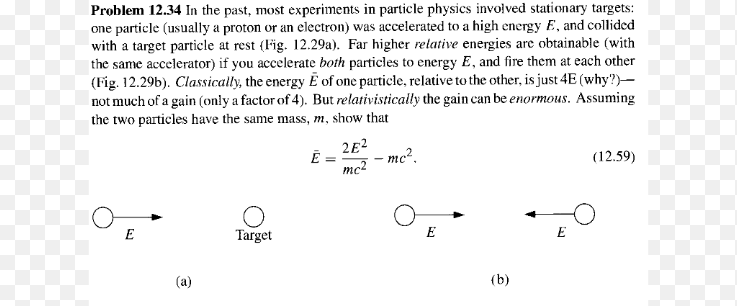
\includegraphics[scale=0.3]{scattering.png}
  \end{center}
\end{frame}

\begin{frame}
  \frametitle{Magnetism is Literally Just Relativity}
  \begin{center}
    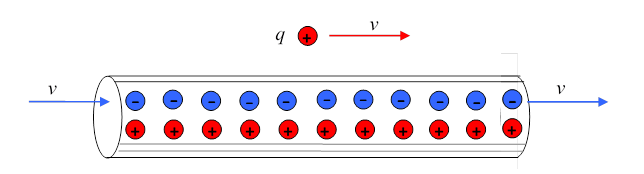
\includegraphics[scale=0.5]{charge.png}
  \end{center}
  Suppose the particle moves to the right at speed $u<v$, the negative charges move to the right at speed $v$, and the positive charges move to the left with speed $v$.
  There ought to be (little to) no net electrical force on the point charge in the frame of the wire, as the charge densities (charge per unit length, in terms of which current is defined) are of equal magnitude.
  However, what happens in the charge's frame?
  We must apply Einstein's velocity addition rule, yielding a line charge velocity of
  \[
    v_{\pm}=\frac{v\mp u}{1\mp vu/c^{2}}
  \]
  Note in particular $v_{-}>v_{+}$, implying the spaces between the charges in the line are wider in the particle's frame, so \textit{it should feel a net electric force in its frame}.

\end{frame}

\begin{frame}
  \frametitle{Magnetism is Literally Just Relativistic Electric Fields in Disguise}
  Moreover, one can prove using the relativistic dynamics that the magnitude of the electric force in the particle's frame is \textit{identical to the classical expression of the magnetic field on a moving line charge}.
  The ``primitive object'' of the usual theory of magnetism are these line currents, so \textit{all} magnetism is attributable to this relativistic effect.
  This is so deeply profound it bears explicit statement: \textbf{\textit{magnetic forces are nothing more than electric forces in the moving frame of the charge they affect}}.
  \footnote{An introductory text that describes magnetism from this perspective \textit{ab initio} (and more carefully) is Purcell's \textit{Electricity and Magnetism}.}
\end{frame}

\begin{frame}
  \frametitle{Elegant Closure}
  Maxwell's equations prettify greatly if one exploits this fact by writing them in a Lorentz-invariant form.
  We will proceed in much lighter detail due to much greater technicality.
  Before Einstein, many attempts were made to unify all four of Maxwell's equations into a single one.
  Most used some sort of tensorial description, to some success, as illustrated by the elegant expression for the electrical force on an arbitrary, time-varying charge configuration in an enclosing volume $V$ due to Maxwell himself:
  \[
    \vec{F}=\int_{\partial V}T_{ij}\cdot d\vec{a}-\epsilon_{0}\mu_{0}\frac{d}{dt}\int_{V}\vec{S}d\tau
  \]
  $T_{ij}$ is the so-called ``Maxwell stress tensor'', an object of a type we'll soon define leading to the final, power-level-9000 form of the laws governing classical electromagnetism.
\end{frame}

\begin{frame}
  \frametitle{Elegant Closure: Defining Tensors}
  Physicists and mathematicians disagree on what tensors are.
  Unfortunately, physicists' definition is objectively worse by orders of magnitude.
  \begin{mydef}
    \textit{A tensor is a multilinear functional on arbitrary copies of a vector space or its dual  (the vector space of 1-forms), i.e. a map, linear in each argument, of the form} $f:V\times\cdots\times V\times V^{*}\times\cdots V^{*}\to \mathbb{F}$
  \end{mydef}
  Physicists get confused because many of their tensors don't look like they produce scalars.
  The aforementioned Maxwell stress tensor seems to produce a vector, the traction, but we can always say the tensor also takes as an argument a 1-form over which the output vector is integrated to produce a scalar,
  or another vector with which the output vector is dotted (canonical isomorphism between $V$ and $V^{*}$).
  In other words, functions that act on vectors to produce a vector are just partial applications of a tensor.
\end{frame}

\begin{frame}
  \frametitle{Elegant Closure: The Four-Potential and Field Tensor}
  The field tensor takes as input a particle's velocity vector and outputs the Minkowski force on the particle due to the magnetic fields, generalizing the electric and magnetic fields into a single object
  that takes in a 4-velocity and outputs the 4-force:
  \[
    F^{\mu\nu}=
    \begin{bmatrix}
      0 & E_{x}/c & E_{y}/c & E_{z}/c \\
      -E_{x}/c & 0 & B_{z} & -B_{y} \\
      -E_{y}/c & -B_{z} & 0 & B_{x} \\
      -E_{z}/c & B_{y} & -B_{x} & 0
    \end{bmatrix}
  \]
  All the information about the scalar and vector potentials $V$ and $\vec{A}$ (which generate the fields by $\nabla V$ and $\nabla\times \vec{A}$, respectively) is contained in the similarly-invariant vector $A^{\mu}=(V/c,A_{x},A_{y},A_{z})$,
  which is related to the field tensor by
  \[
    F^{\mu\nu}=\frac{\partial A^{\nu}}{\partial x_{\mu}}-\frac{\partial A^{\mu}}{\partial x_{\nu}}
  \]
  Charge and current densities are described in this form by
  \[
    J^{\mu}=(c\rho,J_{x},J_{y},J_{z})
  \]
\end{frame}

\begin{frame}
  \frametitle{Elegant Closure: Maxwell's Final Form}
  The last thing we must introduce is a differential operator: the d'Alembertian, $\Box^{2}=\nabla^{2}-\frac{1}{c^{2}}\frac{\partial^{2}}{\partial t^{2}}$ is commonly used to describe wave phenomena, as the wave equation can be written $\Box^{2} u=0$.
  We can now describe all of electromagnetism in a single, two-term partial differential equation:
  \begin{center}
    \boxed{\Box^{2}A^{\mu}=-\mu_{0}J^{\mu}}
  \end{center}
\end{frame}

\begin{frame}
  \frametitle{Looking Forward}
  Relativistic electrodynamics lays the groundwork for general relativity by casting problems in this covariant, coordinate-independent light.
  This language is readily generalized to that of Hodge operators and differential forms:
  \[
    d\star dA = \mu_{0}J
  \]
  similarly contains all the information of Maxwell's equations.

  Hints of quantum mechanics pervade it as well: we know photons to be massless and move at the speed of light.
  The relativistic energy and momentum are \textit{indeterminate} in this case---0/0.
  Therefore, the existence of lightspeed, massless particles that carry momentum and energy is consistent with relativity, but requires \textit{new physics} to explain it.
  That physics came courtesy Planck, who kicked off quantum mechanics by establishing $E=h\nu$ for photons.

  Conclusion: special relativity is unbelievably goated.

\end{frame}

\end{document}
%%% Local Variables:
%%% mode: latex
%%% TeX-master: t
%%% End:
